\documentclass{article}
\usepackage{graphicx} % new way of doing eps files
\usepackage{listings} % nice code layout
\usepackage[usenames]{color} % color
\definecolor{listinggray}{gray}{0.9}
\definecolor{graphgray}{gray}{0.7}
\definecolor{ans}{rgb}{1,0,0}
\definecolor{blue}{rgb}{0,0,1}
% \Verilog{title}{label}{file}
\graphicspath{ {H:/ELC3338/Team8/CompOrg_Spring2018_S1_Team8/images/} }
\newcommand{\Verilog}[3]{
  \lstset{language=Verilog}
  \lstset{backgroundcolor=\color{listinggray},rulecolor=\color{blue}}
  \lstset{linewidth=\textwidth}
  \lstset{commentstyle=\textit, stringstyle=\upshape,showspaces=false}
  \lstset{frame=tb}
  \lstinputlisting[caption={#1},label={#2}]{#3}
}


\author{Matthew Carrano and Breana Leal}
\title{Lab 12: Full Non-Pipelined Datapath}

\begin{document}
\maketitle

\section{Introduction}
The goal of the lab is to integrate all five stages of the ARM's datapath into one module. Previously, each stage was implemented as a separate lab assignment and tested for accuracy. The stages are compared with an expected results table, configured with binary instruction sets. As a final test, a new binary data file was created to perform a simple division. 


\section{Interface}
This section should identify the inputs and outputs of each stage.  To do this, rather than explaining them in paragraph form, please take the datapath diagram in Figure ~\ref{fig:datapath} and add your signal names to the diagram.  This will give you a graphical representation of your system that can be quickly evaluated to determine the meaning of each signal.  For any additional signals that appear on your simulation results, put the signals in a table with a short description of that signal.

\begin{figure}
	\caption{Full Non-Pipelined Datapath}\label{fig:datapath}
	\begin{center}
		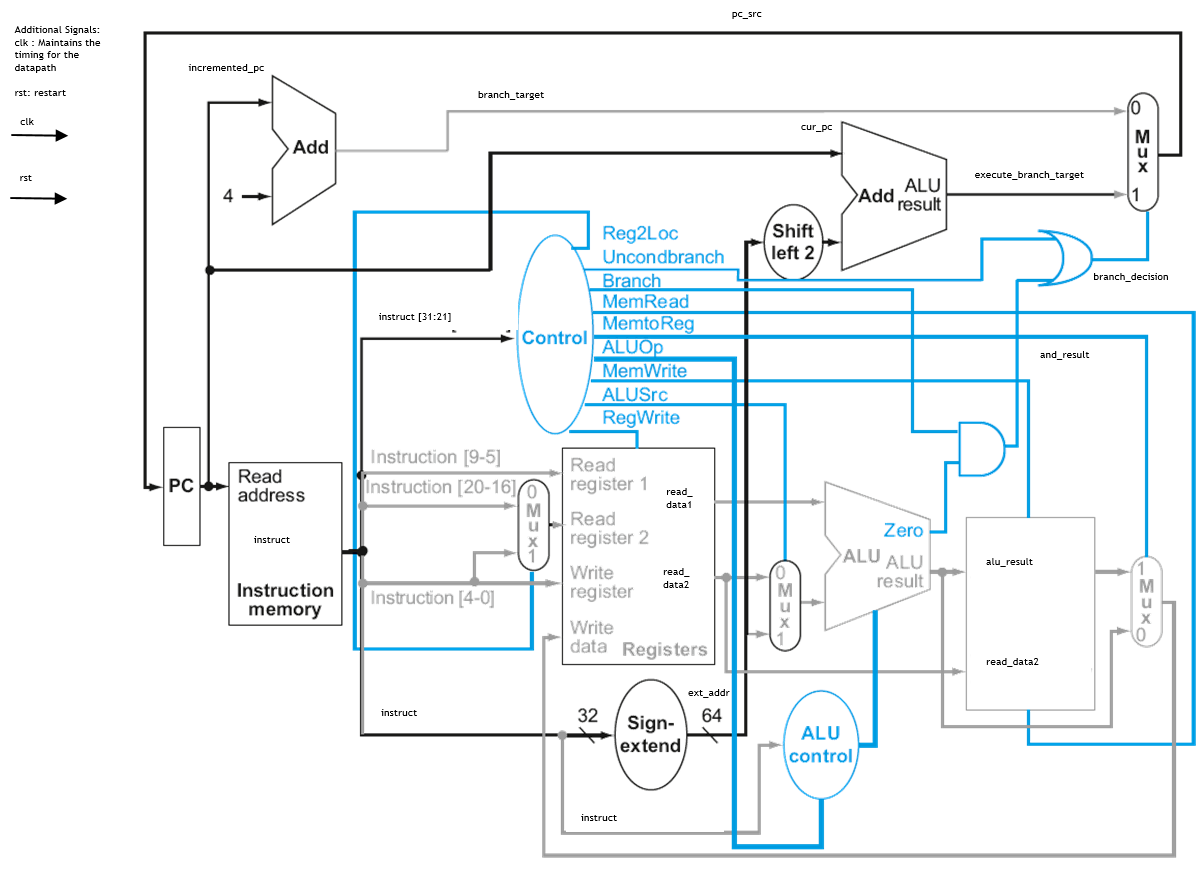
\includegraphics[width=\textwidth]{../images/Picture1.png}
	\end{center}
\end{figure}

\section{Design}
 See Figure ~\ref{fig:timing_diagram_example}
\begin{figure}
	\caption{Timing Diagram }\label{fig:timing_diagram_example}
	\begin{center}
		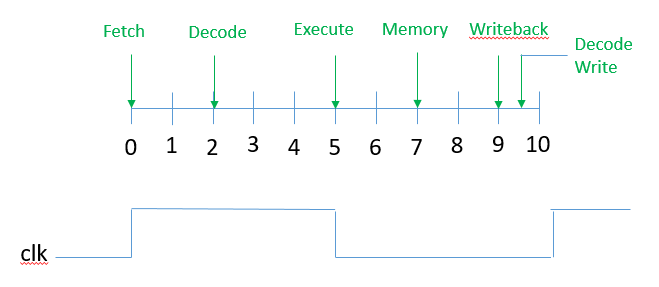
\includegraphics[width=\textwidth]{../images/timing_diagram_example.png}
	\end{center}
\end{figure}

\section{Implementation}
\Verilog{Verilog code for testing the fetch stage.}{code:instrtest}{../code/2_decode/datapath.v} 

\section{Test}
\begin{enumerate}
	\item Assembly code for the "Division Problem" C Code
	For x = X10, y = X11, z = X12, one = X13, Base address of A = X22
	
	 LDUR X10, [X22, \#0]
	 
	 LDUR X11, [X22, \#8]
	 
	 LDUR X12, [X22, \#16]
	 
	 LDUR X13, [X22, \#24]
	 
	 SUB X10, X10, X11
	 
	 ADD X12, X12, X13
	 
	 B -3
	 
	 STUR X12, [X22,\#16]
	
	\item Instruction Data File for the Division Problem
	
	See Figure ~\ref{fig:instruction data}
	\begin{figure}
		\caption{Instruction Data}\label{fig:instruction data}
		\begin{center}
		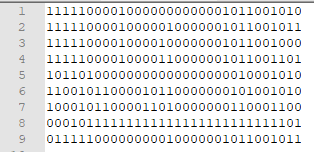
\includegraphics[width=\textwidth]{../images/instra_data2.png}
	\end{center}
\end{figure}

	\item Register Data File for the Division Problem
	
	See Figure ~\ref{fig:ram data}
	\begin{figure}
		\caption{Ram Data}\label{fig:ram data}
		\begin{center}
		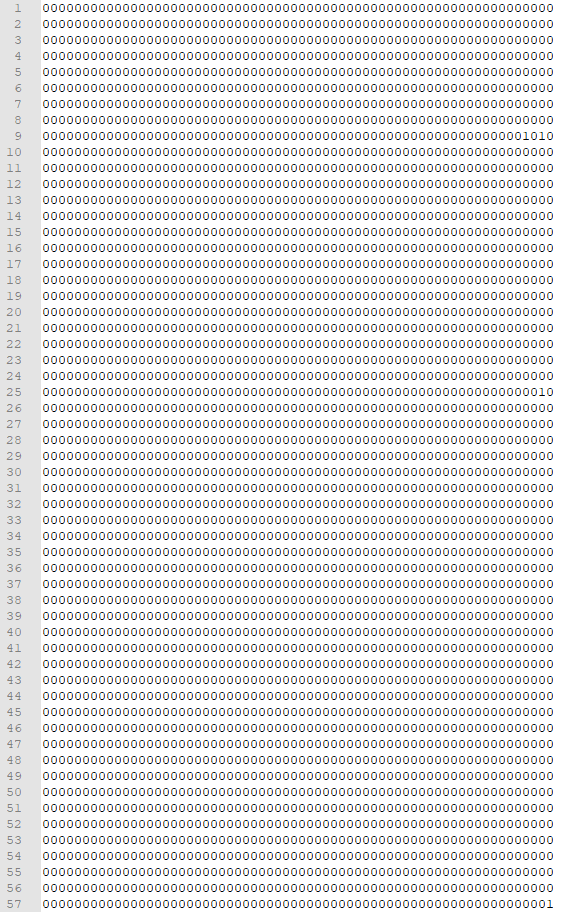
\includegraphics[width=\textwidth]{../images/ram_data2.png}
	\end{center}
\end{figure}

	\item Memory Data File for the Division Problem
	
	See Figure ~\ref{fig:register file}
	\begin{figure}
		\caption{Register File}\label{fig:register file}
		\begin{center}
		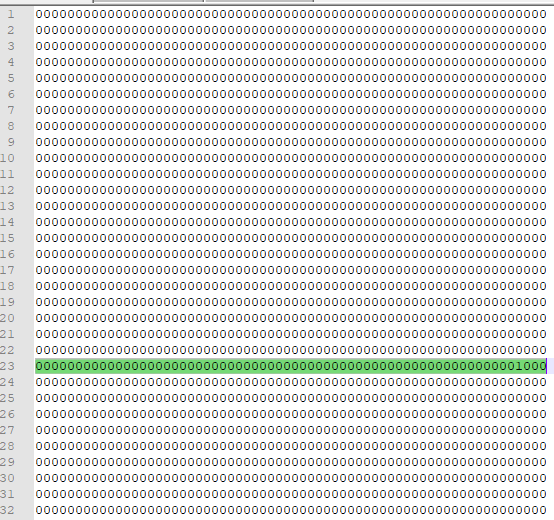
\includegraphics[width=\textwidth]{../images/reg_data2.png}
	\end{center}
\end{figure}

	\item Simulation Results for the Division Problem
	
	See Figure ~\ref{fig:div sim}
	\begin{figure}
		\caption{Division Simulation}\label{fig:div sim}
		\begin{center}
		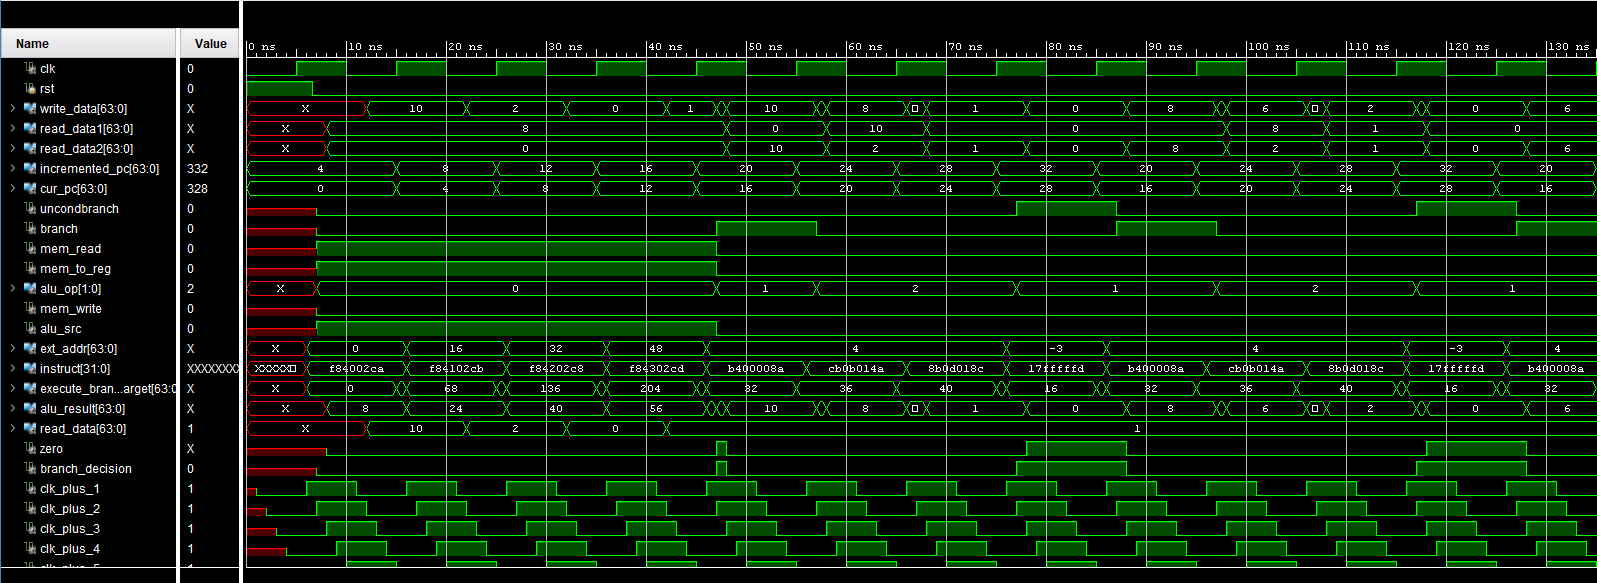
\includegraphics[width=\textwidth]{../images/div_sim_1.png}
		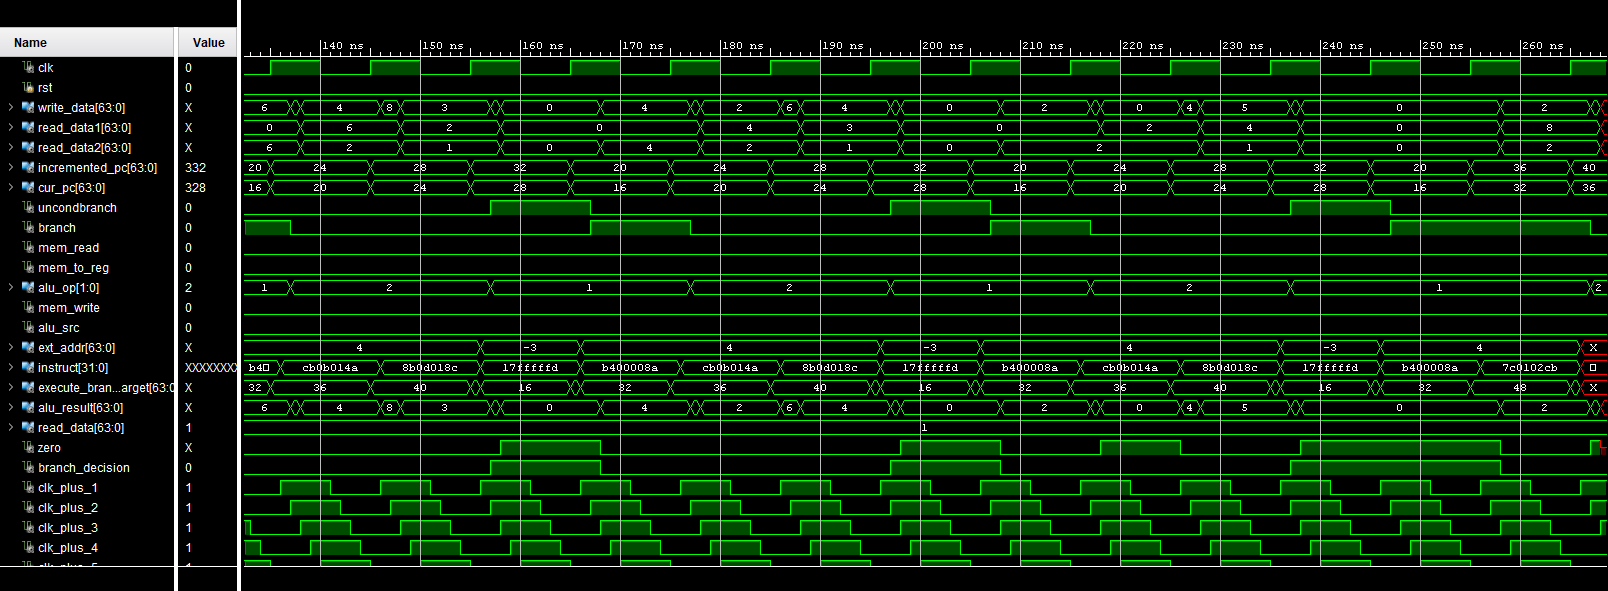
\includegraphics[width=\textwidth]{../images/div_sim_2.png}
	\end{center}
\end{figure}

\end{enumerate}

\section{Conclusions}
Our datapath is working successfully based on our results from the division code. The code divided 10 by 2. The program looped through six times, attaining a correct final alu\_result of 5. The value was then stored in A[2].
\end{document} 